%%%%%%%%%%%%%%%%%%%%%%%%%%%%%%%%%%%%%%%%%%%%%%%%%%%%%%%%%%%%%%%%%%%%%%%%%%%%%%%%
%Objetivo: Introduzir os conceitos envolvidos na dissertação bem como do
%trabalho realizado.  A ideia é que qualquer pessoa que leia a introdução
%consiga ter uma visão geral sobre a dissertação.
%Autor: Vagner Clementino<vagnercs@dcc.ufmg.br> e
%		Rodolfo Resende<rodolfo@dcc.ufmg.br>
%Criação: Dom Set 18 22:55:43 BRT 2016
%Modificação: Dom Set 25 15:41:09 BRT 2016
%Revisão: Dom Set 25 15:41:39 BRT 2016
%%%%%%%%%%%%%%%%%%%%%%%%%%%%%%%%%%%%%%%%%%%%%%%%%%%%%%%%%%%%%%%%%%%%%%%%%%%%%%%%
\chapter{Introdução}
\label{ch:intro}

Dentro do ciclo de vida de um produto de software o processo de manutenção tem
papel fundamental. Devido ao seu alto custo, em alguns casos chegando a 60\% do
preço final~\cite{kaur2015review}, as atividades relacionadas a manter e evoluir
software têm sua importância considerada tanto pela comunidade científica quanto
pela indústria.

Desde o final da década de 1970~\cite{Zelkowitz:1979:PSE:578504} percebe-se o
aumento do custo referente as atividades de  manutenção de software. Nas décadas
de 1980 e 1990 alguns trabalhos tiveram seu foco no desenvolvimento de modelos
de mensuração do valor necessário para manter o
software~\cite{Herrin:1985:SMC:323287.323383,hirota1994approach}. Apesar da
evolução das metologias de manutenção a estimativa é que nas últimas duas
décadas o custo de manutenção tenha aumentado em
50\%~\cite{koskinen2010software}. Esta tendência pode ser observada na
Figura~\ref{fig:software-maintence-costs} onde é possível verificar a evolução
dos gastos com manutenção de software como fração do preço final do produto.

\begin{figure}[htpb]
\centering
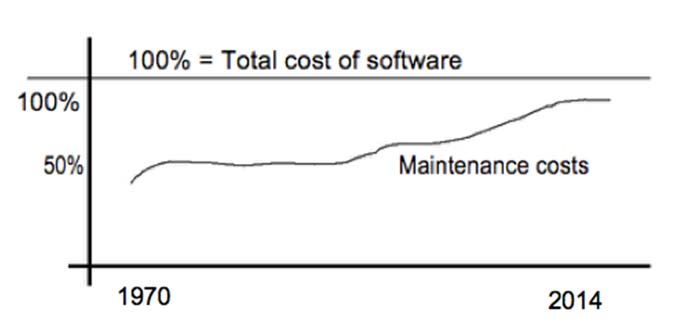
\includegraphics[width=0.7\linewidth]
				{./chapter-intro/img/software-maintence-costs.png}
\caption{Evolução da manutenção de software como percentual do custo total.
	Extraído de~\cite{engelbertink2010save}}
\label{fig:software-maintence-costs}
\end{figure}

Uma vez que o software entra em operação, anomalias são descobertas, mudanças
ocorrem do ambiente de operação e novos requisitos são solicitados pelo usuário.
Todas estas demandas devem ser solucionadas na fase de Manutenção que inicia com
entrega do sistema, entretanto, alguns autores defendem que certas atividades,
como aquelas relativas à analise da qualidade, começam bem antes da entrega do
produto.

A \textit{Manutenção}, dentre outros aspectos, corresponde ao processo de
modificar um componente ou sistema de software após a sua entrega com o objetivo
de \textit{corrigir falhas, melhorar o desempenho ou adaptá-lo devido à mudanças
	ambientais}~\cite{{159342}}. De maneira relacionada,
\textit{Manutenibilidade} é a propriedade de um sistema ou componente de
software em relação ao grau de \textit{facilidade} que ele pode ser corrigido,
melhorado ou adaptado~\cite{{159342}}.

Verificamos na literatura uma discussão sobre a diferença entre manutenção e
evolução de software. Percebe-se ainda que pesquisadores e profissionais
utilizam evolução como o substituto preferido para
manutenção~\cite{Bennett:2000:SME:336512.336534}. Todavia, não está no escopo
desta dissertação discutir e apresentar as diferenças entre os conceitos. Neste
sentido, utilizamos os termos \textit{manter} e \textit{evoluir} software de
forma intercambiáveis.

As manutenções em software podem ser divididas em \textit{Corretiva, Adaptativa,
	Perfectiva e Preventiva}~\cite{Lientz:1980:SMM:601062,159342}. A ISO 14764
discute os quatro tipos de manutenções e propõe que exista um elemento comum
denominado \textit{Requisição de Mudança} que representa as características
comuns a todas aqueles tipos de manutenção.

Por conta do volume das Requisições de Mudança se faz necessária a utilização de
ferramentas com o objetivo de gerenciá-las. Esse controle é geralmente realizado
por \textit{Ferramentas de Gerenciamento de Requisição de Mudança -~FGRM}, que
auxiliam os desenvolvedores na correção de forma individual ou colaborativa de
defeitos (bugs), no desenvolvimento de novas funcionalidades, dentre outras
tarefas relativas à manutenção de software.  A literatura não define uma
nomenclatura comum para este tipo de ferramenta. Em alguns estudos é possível
verificar nomes tais como Sistema de Controle de Defeito -~Bug Tracking Systems,
Sistema de Gerenciamento da Requisição -~Request Management System, Sistemas de
Controle de Demandas (SCD)- Issue Tracking Systems. Todavia, de modo geral, o
termo se refere as ferramentas utilizadas pelas organizações para \textit{gerir
	as Requisições de Mudança}. Estas ferramentas podem ainda ser utilizadas por
gestores, analistas de qualidade e usuários finais para atividades como
gerenciamento de projetos, comunicação, discussão e revisões de código. Neste
trabalho utilizaremos o termo \texttt{Ferramentas de Gerenciamento de
	Requisições de Mudança} (FGRM) ao referimos a este tipo de ferramenta.  A
Tabela~\ref{tab:exemplo} apresenta alguns exemplos de software que podem ser
classificados como FGRM's. Também são listados serviços da Internet que oferecem
funcionalidades presentes nas FGRM's na forma de Software como
Serviço~\cite{fox2013engineering}.

\begin{table}[ht]
	\centering
	\resizebox{\textwidth}{!}{%
		\begin{tabular}{llll}
			\hline
			\multicolumn{2}{c}{\textbf{Ferramentas}}           & \multicolumn{2}{c}{\textbf{Serviços da Internet}} \\ \hline
			Bugzilla & https://www.bugzilla.org/               & SourceForge    & https://sourceforge.net/    \\ \hline
			MantisBT & https://www.mantisbt.org/               & Lauchpad       & https://launchpad.net/      \\ \hline
			Trac     & https://trac.edgewall.org/              & Code Plex      & https://www.codeplex.com/   \\ \hline
			Redmine  & www.redmine.org/                        & Google Code    & https://code.google.com/    \\ \hline
			Jira     & https://www.atlassian.com/software/jira & GitHub         & https://github.com/         \\ \hline
		\end{tabular}%
	}
	\caption{Exemplos de ferramentas e serviços da Internet. Adaptado
		de~\cite{cavalcanti2014challenges}}\label{tab:exemplo}
\end{table}

\section{Motivação}
\label{sec:intro-motivacao}

Diante da maior presença de software em todos os setores da sociedade existe um
interesse por parte da academia e da industria no desenvolvimento de processos,
técnicas e \textit{ferramentas} que reduzam o esforço e o custo das tarefas de
desenvolvimento e manutenção de software. Nesta linha, o trabalho de Yong \&
Mookerjee~\cite{1423995}  propõe um modelo que reduz os custos de manutenção e
reposição durante a vida útil de um sistema de software. O modelo demonstrou que
em algumas situações é \textit{melhor substituir um sistema do que mantê-lo}.
Este pro\-ble\-ma é agravado tendo em vista que em alguns casos são necessários 
que 60\% dos desenvolvedores fique dedicados à tarefas de manutenção de
sistemas~\cite{Zhang_2003}.

Em certos projetos de software, especialmente durante as etapas de
desenvolvimento e teste, se faz necessário uma ferramenta para gerenciar
as Requisições~de~Mudança por conta do volume e da grande quantidade de pessoas
que necessitam de um local para inserir os erros encontrados~\cite{1407819}.
Este tipo de ferramenta vem sendo utilizada em projetos de código
aberto (Apache, Linux, Open Office) bem como em organizações públicas e privadas
(NASA,IBM).

Não obstante, alguns estudos demonstram que as FGRM's desempenham um papel além
de gerenciar os pedidos de manutenção software. Avaliando o controle de demandas
como um processo social, Bertram e
outros~\cite{Bertram:2010:CCB:1718918.1718972} realizaram um estudo qualitativo
em FGRM's quando utilizados por pequenas equipes de desenvolvimento de software.
Os resultados mostraram que este tipo ferramenta não é apenas um banco de dados
de rastreamento de defeitos, de recursos ou pedidos de informação, mas também
atua como um ponto focal para a comunicação e coordenação de diversas partes
interessadas (stakeholders) dentro e fora da equipe de software. Os clientes,
gerentes de projeto, a equipe envolvida com a garantia da qualidade e
programadores, contribuem em conjunto para o conhecimento compartilhado dentro
do contexto das FGRM's.

No trabalho de Breu e outros~\cite{Breu:2010:INB:1718918.1718973} o foco é
analisar o papel dos FGRM's no suporte à colaboração entre desenvolvedores e
usuários de um software. A partir da análise quantitativa e qualitativa de
defeitos registrados em uma FGRM de dois projetos de software livre foi possível
verificar que o uso da ferramenta propiciou que os usuários desempenhassem um
papel além de simplesmente reportar uma falha: a participação ativa e permanente
dos usuários finais foi importante no progresso da resolução das falhas que eles
descreveram.

Um outro importante benefício da utilização das FGRM é que as mudanças no
software podem ser rapidamente identificada e reportada para os
desenvolvedores~\cite{anvik2005coping}. Além disso, eles podem ajudar a estimar
o custo do software, na análise de impacto, planejamento, rastreabilidade,
descoberta do conhecimento~\cite{cavalcanti2013bug}.

Contudo, no escopo de utilização das FGRM's diversos desafios se apresentam:
duplicação RM's, pedidos de modificação abertos inadvertidamente, grande
volume de RM's que devem ser atribuídas aos desenvolvedores, erros descrito
de forma incompleta, análise de impacto das RM's e RM's atribuídas de maneira
incorreta~\cite{cavalcanti2014challenges}.  Diante de tantos problemas e
desafios é importante entender como estas ferramentas vêm sendo
utilizadas bem como analisar o que está sendo proposta na literatura com objetivo
de melhorar as funcionalidades oferecidas por elas\@.

%No trabalho de Junio et al.~\cite{5741246} é proposto um processo denominado
%PASM (Process for Arranging Software Maintenance Requests) que propõe lidar com
%tarefas de manutenção como projetos de software. Para tanto, utilizou-se
%técnicas de análise de agrupamento (clustering) a fim de melhor compreender e
%comparar as demandas de manutenção. Os resultados demostraram que depois de
%adotar o PASM os desenvolvedores tem dedicado um tempo maior para análise e
%validação. De outra forma, relacionada um menor tempo foi dedicado às tarefas
%de execução e codificação.
%
%No estudo realizado por Bettenburg et al.~\cite{bettenburg2008makes} foi
%desenvolvida uma pesquisa (\textit{survey}) entre desenvolvedores e usuários
%dos projetos Apache\footnote{\url{http://www.apache.org/}},
%Eclipse\footnote{\url{https://www.eclipse.org}} e
%Mozilla\footnote{\url{https://www.mozilla.org}} a fim de verificar o que
%produziria uma boa FGRM\@. Os resultados demonstraram que do ponto de vista dos
%desenvolvedores eram consideradas úteis funcionalidades tais como reprodução do
%erro, rastros de pilhas (stack traces) e casos de testes. A partir deste
%resultado foi construído um protótipo capaz de conduzir os usuários na coleta e
%fornecimento de um maior número de informações úteis para a resolução do
%defeito reportado.
%
%
%Em Zimmermann et al.~\cite{5070993} é discutido a importância de que a
%informação descrita em uma Requisição de Mudança seja relevante e completa a
%fim de que o defeito reportado seja resolvido rapidamente. Contudo, na prática,
%a informação apenas chega ao desenvolvedor com a qualidade requerida após
%diversas interações com o usuário afetado. Com o objetivo de minimizar este
%problema os autores propõe um conjunto de diretrizes para a construção de um
%ferramenta capaz de reunir informações relevantes a partir do usuário e
%identificar arquivos que precisam ser corrigidos para resolver o defeito.
%

%No trabalho de Kononenko et al.~\cite{Kononenko:2014:DED:2591062.2591075} é
%apresentada uma ferramenta denominada \textit{DASH} cujo objetivo é agrupar as
%demandas que são relevantes para as atividades de um desenvolvedor.
%Naturalmente todas as demandas ditas relevantes deveriam estar sob a
%responsabilidade de um mesmo programador. O principal objetivo desta ferramenta
%é aumentar a Consciência Situacional (Situational Awareness) dos
%desenvolvedores. Segundo os autores, o principal ganho do uso da ferramenta é
%que os programadores podem gerenciar melhor o excesso de informação e ficar
%mais ciente da evolução das demais demandas do sistema.
%
%Na ferramenta proposta por Thung et al.~\cite{Thung:2014:DIT:2642937.2648627} o
%foco é na determinação de defeitos duplicados. A contribuição deste trabalho é
%a integração do estado da arte de técnicas não supervisionadas para detecção de
%falhas duplicadas conforme proposto por Runeson et
%al.~\cite{Runeson:2007:DDD:1248820.1248882}. A ferramenta utiliza o Modelo de
%Vetor Espacial (Vetor Space Model) como métrica de similaridade entre os
%defeitos e fornece aos desenvolvedores uma lista de possíveis duplicatas.

%A manutenção não necessariamente exige que o processo de software envolvido
%seja o tradicional. Percebe-se alguns exemplos de adoção das práticas ágeis
%para fins de manutenção e evolução do software~\cite{kajko2009model,
%Heeager2015, Devulapally2015,Naz2016}. Tal tendência não é surpreendente tendo
%em vista que os métodos ``ágeis'' enfatizam características úteis à eficiência
%da implementação de software, tais como desenvolvimento incremental e teste
%contínuo que agregam valor para a evolução e manutenção eficaz de um sistema
%\cite{thomas2006agile}. Dentro desta tendência verifica-se a necessidade de que
%as ferramentas envolvidas no suporte à manutenção de software se adéquem à este
%nova forma de manter software.
%


\section{Problema}
\label{sec:intro-problema}

O desenvolvimento e a manutenção de software envolvem diversos tipos de métodos,
técnicas e ferramentas. Em especial no processo de manutenção, um importante
aspecto são as diversas Requisições de Mudanças que devem ser gerenciadas. Este
controle é realizado pelas FGRM's cujo o uso vem crescendo em importância,
sobretudo, por sua utilização por gestores, analistas da qualidade e usuários
finais para atividades como tomada de decisão e comunicação. Contudo, muitas
daquelas ferramentas são meramente melhores interfaces para um banco de dados
que armazena todos os bugs reportados~\cite{zimmermann2009improving}.

Apesar da inegável importância das FGRM's, percebe-se um aparente desacoplamento
deste tipo de ferramenta com as necessidades das diversas partes interessadas
(stakeholders) na manutenção e evolução de software. A utilização de
\textit{``demanda''} como conceito central para Ferramentas de Gerenciamento de
Requisição de Mudanças (FGRM) parece ser distante das necessidades práticas dos
projetos de software, especialmente no ponto de vista dos desenvolvedores
\cite{Baysal:2013:SAP:2486788.2486957}.

Um exemplo deste desacoplamento pode ser visto no trabalho proposto por Baysal
\& Holme~\cite{baysal2012qualitative} no qual desenvolvedores que utilizam o
Bugzilla\footnote{\url{https://www.bugzilla.org}} relatam a dificuldade em
manter uma compreensão global das RM's em que eles estão envolvidos. Segundo os
participantes seria interessante que a ferramenta tivesse um suporte melhorado
para a Consciência Situacional -~Situational Awareness. Em síntese, eles
gostariam de estar cientes da situação global do projeto bem como das atividades
que outras pessoas estão realizando.

Um outro problema que é potencializado pela ausência de certas funcionalidades
nas FGRM são as RM's que acabam sendo relatadas de forma insatisfatória. Nesta
situação os usuários acabam sendo questionados a inserir maiores detalhes que
muitas vezes eles não tem conhecimento. Por outro lado, verifica-se uma
frustração por parte dos desenvolvedores que acabam desapontados sobre a
qualidade do que foi reportado~\cite{just2008towards}.

Com o objetivo de melhorar as FGRM's, que no contexto do trabalho recebem o nome
de issue tracking system, Zimmermann e outros
discute~\cite{zimmermann2009improving} quatro dimensões de melhorias deste tipo
de ferramenta, conforme listado a seguir e esquematizado na
Figura~\ref{fig:dimensoes_melhorias_fgrm}. Estas dimensões de melhorias são
descritas com maior detalhe no Capítulo~\ref{ch:mapeamento-sistematico} onde foi
utilizado para a classificação de estudos através do Mapeamento Sistemático
realizado.

\begin{enumerate} [(i)]
	\item{Informação}
	\item{Processo}
	\item{Usuário}
	\item{Ferramenta}
\end{enumerate}

\begin{figure}[htpb] \centering
	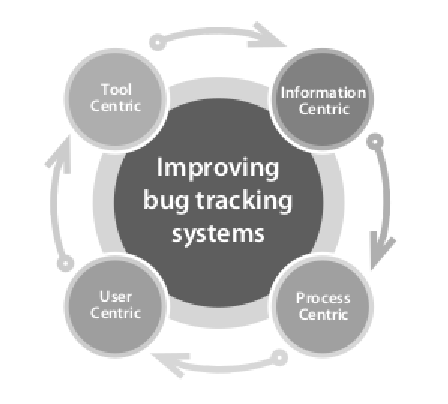
\includegraphics[width=0.666666\linewidth]
	{chapter-intro/img/dimensoes_melhorias_fgrm.pdf}
	\caption{Dimensões de melhoria das FGRM's. Adaptado
		de~\cite{zimmermann2005mining}}\label{fig:dimensoes_melhorias_fgrm}
\end{figure}

Neste estudo estamos especialmente interessados em analisar e propor melhorias
relativas ao domínio da \textit{Ferramenta}. Ao bem do nosso conhecimento é
reduzido o número de trabalhos que avaliem de forma sistemática as
funcionalidades oferecidas pelas FGRM ao mesmo tempo que faça relação com que
vem sendo proposto na li\-te\-ra\-tu\-ra sobre o assunto. De maneira similar o
número de estudos que avaliam a opinião dos profissionais envolvidos em
manutenção de software sobre o que é ofertado pelas FGRM\@.

Além disso, os estudos anteriormente propostos não discutem o fato que da mesma
forma que ocorre no desenvolvimento de software, é possível verificar uma
crescente adoção de técnicas da metodologia ágil na manutenção de
software~\cite{Soltan2016,Devulapally2015, Heeager2015}. Neste contexto, seria
importante que ferramentas que dão suporte à manutenção, tal como as FGRM's,
evoluíssem para se adaptar a esta nova forma de trabalhar. Mesmo em um
ambiente tradicional de  desenvolvimento e manutenção de software, verifica-se a
necessidade de adequação das FGRM's, o que pode ser observado considerando as
diversas extensões (plugins) propostas na literatura
\cite{101186,Thung:2014:BIT:2635868.2661678,Kononenko:2014:DED:2591062.2591075}.

\section{Objetivos}
\label{sec:intro-objetivos}

Conforme exposto o distanciamento entre as necessidades dos profissionais
envolvidos em manutenção de software e as funcionalidades oferecidas pelas FGRM
resulta em diversos problemas. Neste contexto, este trabalho de dissertação
investiga e contribui no entendimento de como as Ferramentas de Gerenciamento de
Requisição de Mudança estão sendo melhoradas ou estendidas no contexto da
transformação do processo de desenvolvimento e manutenção de software de um
modelo tradicional para outro que incorpora cada vez mais as práticas propostas
pelos agilistas. O intuito é analisar como as FGRM estão sendo modificadas com
base na literatura da área em contraste com o ponto de vista dos profissionais
envolvidos em manutenção de software.

Neste contexto, elaboramos um estudo sobre as Ferramentas de Gerenciamento de
Requisição de Mudança (FGRM) com os seguintes objetivos:
\begin{enumerate}[(i)]
	\item entender os requisitos comuns deste tipo de ferramenta;
	\item mapear as extensões para as FGRM que estão sendo propostas na
		literatura;
	\item avaliar sobre o ponto de vista dos profissionais a
		situação atual dos FGRM\@;
	\item propor melhorias ou novas funcionalidades para as FGRM\@.
\end{enumerate}

%Vamos discutir os aspectos que são considerados mais importantes a partir da
%literatura da área, bem como do ponto de vista de profissionais envolvidos em
%manutenção de software. De forma particular, iremos estudar os mecanismos de
%personalização que algumas destas ferramentas permitem e tentaremos ainda criar
%exemplos de personalização para alguma possível extensão a ser identificada ao
%longo do trabalho.

\section{Visão Geral do Estudo}
\label{sec:intro-visao-geral}


A fim de alcançarmos os objetivos descritos na seção anterior, um conjunto de
melhorias nas funcionalidades das FGRM's foi proposto. As melhorias resultaram
de três estudos empíricos: um mapeamento sistemático da literatura, apresentado
no Capítulo~\ref{ch:mapeamento-sistematico}, uma caracterização das
funcionalidades das FGRM, discutida no Capítulo~\ref{ch:caracterizacao}; e uma
pesquisa com profissionais, apresentada no
Capítulo~\ref{ch:pesquisa-profissionais}.

Mediante o mapeamento sistemático obtivemos e avaliamos o estado da arte sobre
novas funcionalidades bem como melhorias no escopo das FGRM\@. A partir do
estudo foi possível propor quatro esquemas de classificação: por tipo de
problema, por suporte ao papel desempenhado na manutenção de software, por
técnicas de Recuperação da Informação utilizada e por ferramenta
estendida.

De maneira similar, através da caracterização das funcionalidade de algumas
FGRM's código aberto ou disponíveis comercialmente e escolhidas mediante uma
pesquisa com profissionais identificamos o estado da prática deste tipo de
ferramenta.

Com base dois estudos anteriores conduzimos uma pesquisa com profissionais
envolvidos em manutenção de software onde pedimos que avaliassem os requisitos
funcionais e não funcionais que poderiam melhorar as FGRM já existentes. O
questionário também quis saber a opinião dos profissionais sobre a relevância
das propostas de me\-lho\-ri\-as existente na literatura em sua rotina de
trabalho.

\section{Metodologia de Pesquisa}
\label{sec:intro-metodologia}

A metodologia de pesquisa utilizada neste estudo é baseada em uma abordagem
multi-método~\cite{hesse2010mixed}. Este tipo de desenho  combina dois ou mais
métodos quantitativo (ou qualitativo) em um único estudo. Um estudo que faça uso
de um survey e um experimento é um exemplo deste tipo de
enfoque~\cite{hesse2010mixed}.

Alguns estudos descrevem quatro tipos de desenho em abordagens multi-método:
embutido (embedded), exploratória, triangulada e
explanatória~\cite{creswell2007designing}. Neste estudo, utilizamos uma
abordagem de triangulação no qual consolidamos os resultados de diferentes
métodos, considerando, contudo, que a mesma questão de pesquisa foi investigada
em cada um deles. A utilização de um desenho triangular no trabalho melhora as
conclusões e completude do estudo, trazendo maior credibilidade para os achados
da pesquisa~\cite{hesse2010mixed}.

As etapas do trabalho, que compõem a abordagem multi-método estão listadas a
seguir:

\begin{itemize}[(i)]
	\item Mapeamento Sistemático da Literatura~\cite{Petersen2008}
	\item Caracterização das Ferramentas de Gerenciamento de Requisição de
		Mudança (FGRM)
	\item Pesquisa (Survey) com os
		desenvolvedores~\cite{wohlin2012experimentation}
%	\item Desenvolvimento de extensões para as FGRM's
\end{itemize}

\section{Contribuições do Estudo}
\label{sec:intro-contribuicao}
Este estudo sistematiza a literatura sobre melhorias das funcionalidades das
FGRM's ao mesmo tempo que avalia junto aos profissionais as relevâncias de tais
alterações. Este estudo ainda se propões este tipo de software por meio de uma
caracterização de suas funcionalidades. Ao final deste trabalho teremos um
conjunto de funcionalidades que podem ser implementadas neste tipo de software
de modo melhorá-lo. 

%\section{Organização do Trabalho}
%\label{sec:intro-organizacao-dissertacao}
%\todo[inline]{Vamos aguardar o desenvolvimento deste trabalho para definirmos a
%estrutura do texto.}
